\chapter{PKiKP/PcP Amplitude Ratio and CMB variation}

利用PKiKP和PcP相位的振幅比可以约束ICB的密度变化和剪切波速度差等性质~\citep{Koper2004a},即
认为PcP和PKiKP在地幔中的射线路径比较接近,则地幔对振幅观测的影响效应可以大部分被消除,同时也可以
避免由于仪器造成的绝对振幅测量不准确的影响,对振幅比异常的贡献主要来自与内核。但这其中隐含了使用
幅比方法研究ICB的一个重要的假设,即核幔边界的性质和结构能比较好的确定且其变化对PKiKP/PcP的振幅
比不敏感。否则,可能会观测到异常大或异常小的PKiKP和PcP振幅比,这样就很难对ICB的性质进行约束。

通过对265对观测到PKiKP相位的事件和台阵对数据的挑选,得到了这两个相位能同时被观测到的111对事件和
IMS台阵的数据,在这个数据集中,两个相位的最大振幅都能较为可靠地被测量。同时,为了探求是什么因素影响
PKiKP和PcP是否同时被观测到,对地震震源参数、震中距和PcP在CMB的反射点位置分布做了一些分析(图
\ref{dep_mag_hist}、图\ref{dis_hist})。从结果来看,对于已有的全部数据,不管是地震的震级、
震源深度还是震中距都不会对这两个相位是否被同时观测到产生太大影响。5.0级之上的事件都可产生清晰
的PcP和PKiKP,这些事件基本集中在0-100km的浅源深度,这也说明在最初对事件的选择不加太多限制是
正确的,较多的5级浅源地震保证了有效数据的数量。

\begin{figure}[!ht]
	\centering
	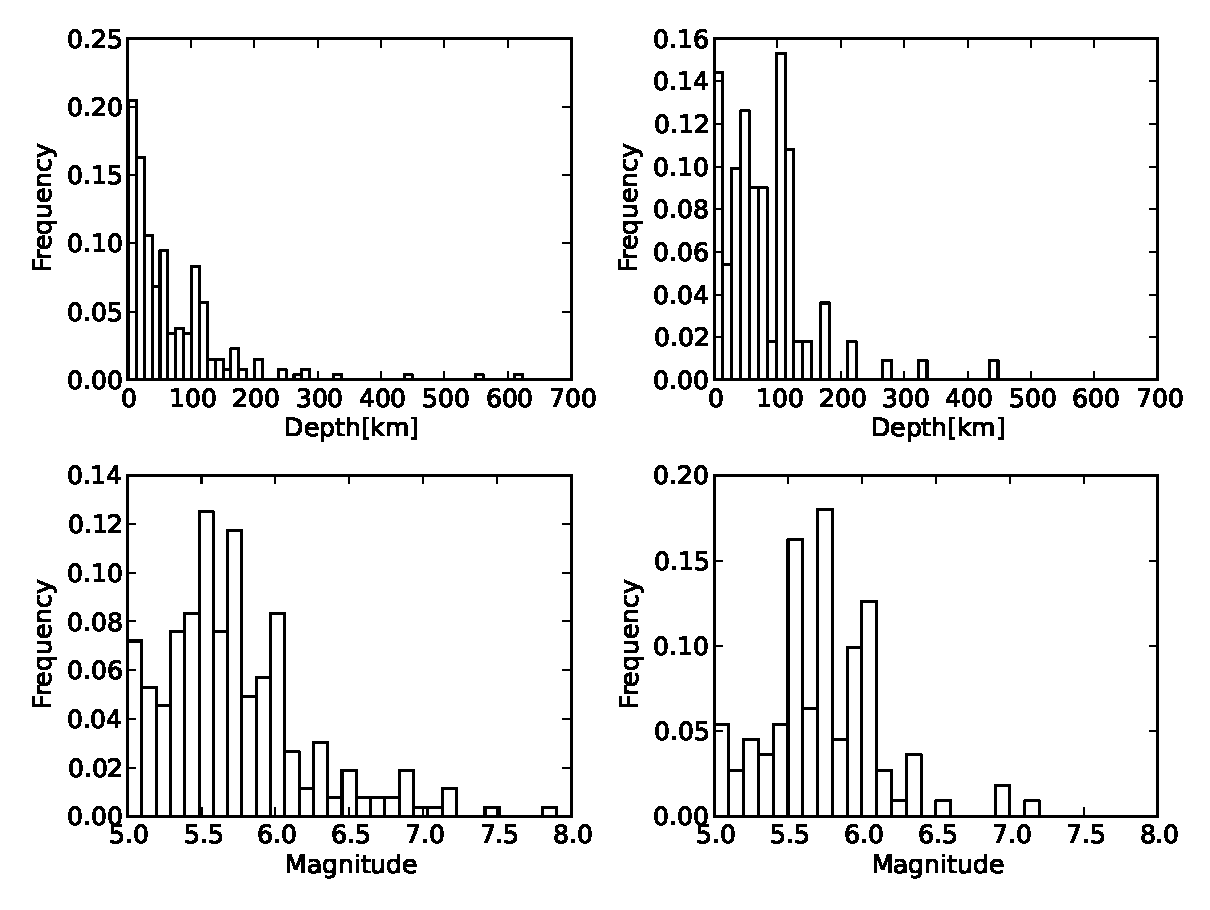
\includegraphics[width=12cm,height=9cm]{fig/chap4/depmag_hist.eps}
	\caption{(a),(b)分别为观测到PKiKP相位的事件和同时观测到PcP和PKiKP的事件随震源深度%
的分布;(c),(d)分别为观测到PKiKP相位的事件和同时观测到PcP和PKiKP的事件随震级的分布。}
	\label{dep_mag_hist}
\end{figure}

\begin{figure}[!ht]
	\centering
	\includegraphics[width=12cm,height=4.5cm]{fig/chap4/dist_hist.eps}
	\caption{(a),(b)分别为观测到PKiKP相位的事件和同时观测到PcP和PKiKP的事件随震中距%
的分布。}
	\label{dis_hist}
\end{figure}

由于震源深度并不对PKiKP和PcP的可观测性产生较大影响,因此可以很大程度上排除未观测到PcP但观测到
PKiKP是上地幔结构的影响,比如上地幔低速带对PcP振幅的衰减作用。这就更加强烈的暗示了核慢边界的性质
是影响PcP相位观测的主要因素,也说明了CMB结构对PKiKP/PcP振幅比也可能产生巨大影响。从观测和
未观测到的PcP在CMB反射点的分布来看(图\ref{loc_distri}),即使在某个区域内,CMB的性质也可能发生强烈变化(即图中蓝色和红色的交替出现)。

\begin{figure}[!ht]
	\centering
	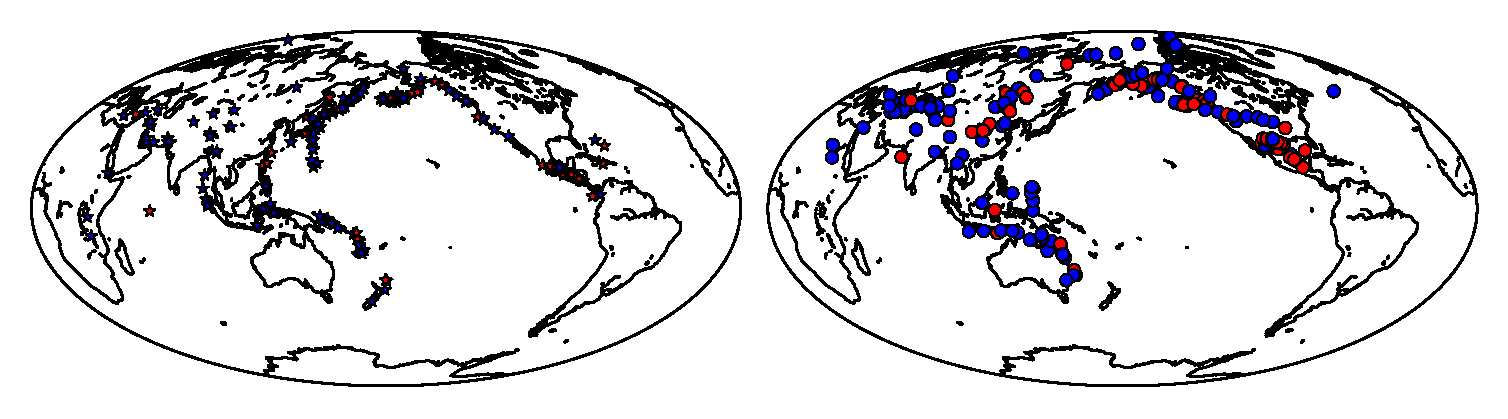
\includegraphics[width=12cm,height=4cm]{fig/chap4/loc_distri.eps}
	\caption{左图为地震事件的分布,红色五角星表示同时观测到PKiKP和PcP的事件,蓝色五角星表示%
仅观测到PKiKP的事件;右图为PcP在CMB的上的反射点分布,红色圆圈表示同时观测到PKiKP和PcP,蓝色%
圆圈表示仅观测到PKiKP的反射点。}
	\label{loc_distri}
\end{figure}

\section{Local intensive variation of CMB property}

之前的观测已经表明CMB的横向变化会产生异常大的PKiKP/PcP振幅比~\citep{Koper2004a},且是理论预
期的振幅比的数倍。产生异常大的振幅比是因为PcP的振幅异常小,即在由CMB反射的PcP的振幅受到很大的损
失。可能的解释有(1)下地幔底部存在超低速带;(2)核幔边界存在厚的转换带~\citep{Garnero2000}。当
转换带的厚度接近入射波的波长的时候,反射系数会剧烈减小~\citep{richards1972};(3)核慢边界的地
形起伏。地形起伏产生的聚焦和散焦效应会产生异常的PcP振幅~\citep{Neuberg1991}。很难用只用这三
种解释中的一种来解释与理论振幅比相差达到十倍的观测数据,因此异常的PcP振幅很可能是多种因素的共同
的结果。图\ref{nvar_ratio_cor}和图\ref{pdar_ratio_cor}显示了NVAR台阵和PDAR台阵观测的PK
iKP/PcP振幅比分别与PcP、PKiKP振幅的关系。NVAR台阵数据中,PKiKP/PcP震幅比和PcP的振幅显示出强
烈的负相关,而与PKiKP振幅则没有明显关系,表明在NVAR数据采样到的CMB区域可能存在强烈的横向变化;而
对于PDAR台阵,振幅比与PcP的相关性则略小,但振幅比则普遍较NVAR台阵偏高,可能在这部分数据采样的CMB
性质横向变化较弱,且采样区域可能位于低速带中。

\begin{figure}[!ht]
	\centering
	\includegraphics[width=12cm,height=4.5cm]{fig/chap4/nvar_ratio_cor.eps}
	\caption{NVAR台阵观测到的PKiKP/PcP振幅比和PcP振幅的关系,其中PcP的振幅用对数坐标表%
示。}
	\label{nvar_ratio_cor}
\end{figure}

\begin{figure}[!ht]
	\centering
	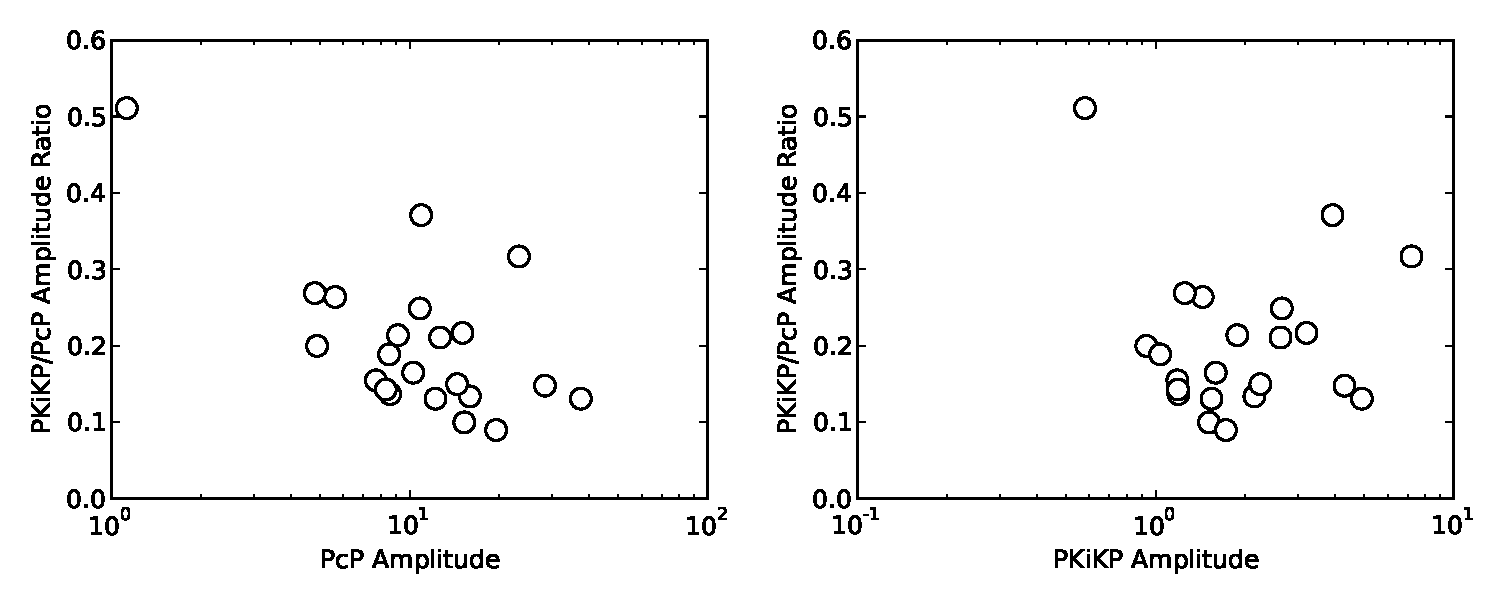
\includegraphics[width=12cm,height=4.5cm]{fig/chap4/pdar_ratio_cor.eps}
	\caption{PDAR台阵观测到的PKiKP/PcP振幅比和PcP振幅的关系,其中PcP的振幅用对数坐标表%
示。}
	\label{pdar_ratio_cor}
\end{figure}

\subsection{Varify CMB effects on Amplitude Ratio}

在111对同时观测到较清晰的PcP和PKiKP的事件-台阵数据集中,有22个地震事件被一个以上的IMS台阵记录
到,这就为检验核慢边界横向变化对PKiKP/PcP振幅比的影响提供了绝佳的条件。还是以NVAR和PDAR两个台
阵为例,在22个事件中由这两个台阵同时观测到的就有10个,震中距都在25{\textdegree}以上,且其中
7个都在31-34{\textdegree}之间,这些事件全都来自墨西哥—危地马拉的地震带,震源位置都比较接近,
震源深度的差别也不是很大。这十个事件见表\ref{nvpd}。通过对比可以发现,不同台阵观测到的PKiKP/Pc
P振幅比可以有巨大的差别,对有的事件NVAR和PDAR两个台阵观测到的振幅比差别竟然能达到10倍之多,而且
在后面的讨论中可以看出这绝不是偶然的情况,在相同的观测频率下(1-2Hz),如此大的差别很难想象是由除C
MB横向变化之外的其他因素所造成,因为两个台阵到事件的震中距差别不大,NVAR和PDAR也只相距1000公里,
同一事件在内核的反射点在内核表面的距离也小于它们对应于CMB反射点的距离;对某些事件,两个台阵的观测
的振幅比则极为接近,可能这部分事件的数据采样到CMB性质相近的区域。

\begin{table}[!ht]
	\centering
	\begin{tabular}{*{3}{l}*{2}{c}*{2}{l}}
	\hline
	n & Date & Hour & Latitude & Longitude & Depth & Magnitude\\
	\hline
1 & 2003/08/25 & 06:28:34.9 &  13.9932 &  -91.1255 &  99.5 & 5.9\\
2 & 2007/07/23 & 22:30:09.2 &  14.465  &  -90.906  &  115  & 5.5\\
3 & 2009/11/26 & 19:08:10.4 &  13.4767 &  -89.9617 &  48.5 & 5.9\\
4 & 2009/04/27 & 16:46:27.5 &  16.9557 &  -99.5717 &  31.7 & 5.8\\
5 & 2009/05/03 & 16:21:46.4 &  14.6199 &  -91.2025 &  113.9 & 6.3\\
6 & 2009/08/15 & 13:22:43.1 &  18.0998 & -100.6157 &  61.2 & 5.5\\
7 & 2012/06/27 & 06:30:59.8 &  13.834  &  -89.967  &  132.6 & 5.7\\
8 & 2012/11/15 & 09:20:21.9 &  18.346  & -100.382  &  53  & 6.1\\
9 & 2013/07/08 & 02:52:42.6 &  13.2316 &  -89.1292 &  55  & 5.7\\
10 & 2014/01/11 & 13:10:51.1 &  14.6437 &  -92.0592 &  78  & 5.5\\
	\hline
\end{tabular}
	\caption{同时观测到PKiKP和PcP的事件—台阵对数据中同时被NVAR和PDAR台阵观测到的10个事件%
。}
	\label{nvpd}
\end{table}

\begin{figure}[!ht]
	\hfill{}
	\subfloat[]{\centering%
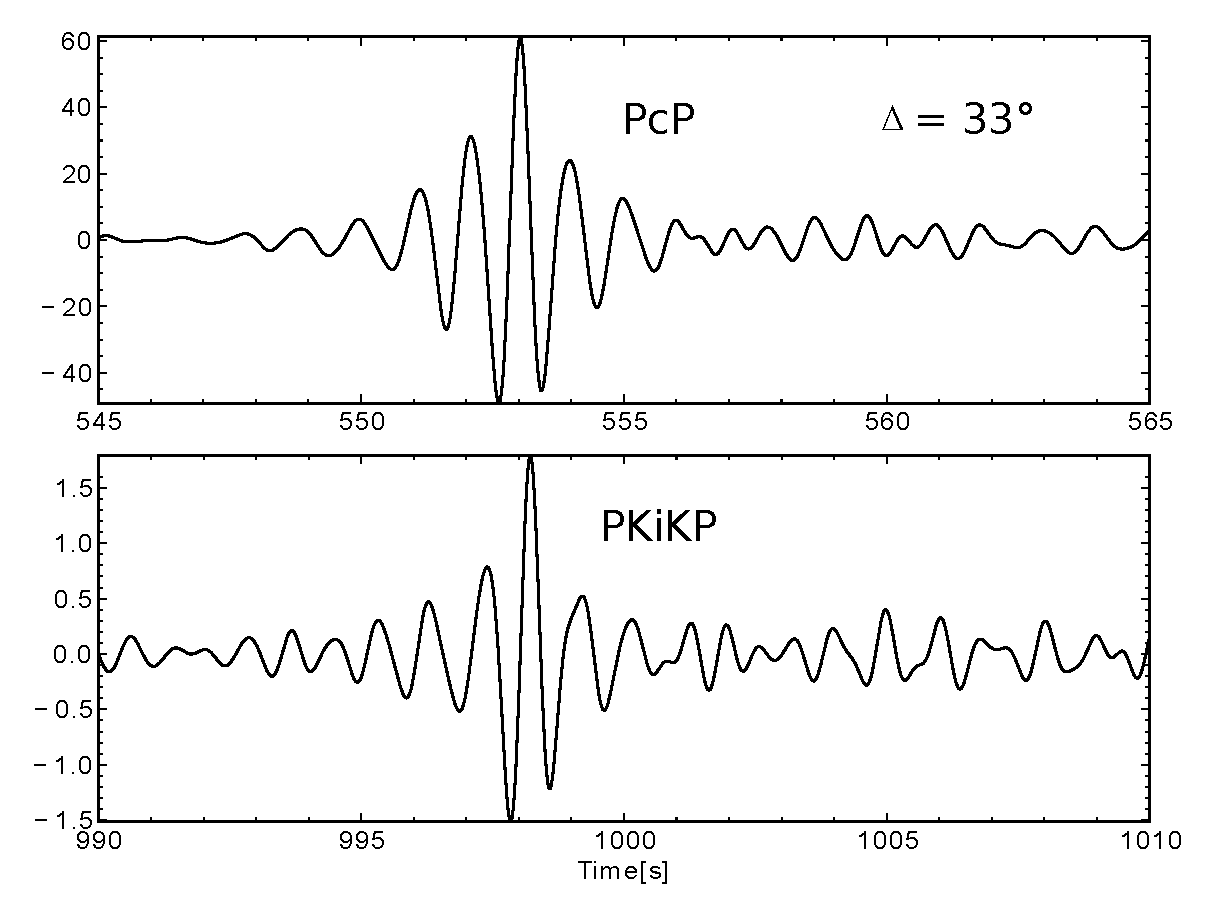
\includegraphics[width=8cm,height=8cm]{fig/chap4/amp_nv_4371355.eps}
}
	\hfill{}
	\subfloat[]{\centering%
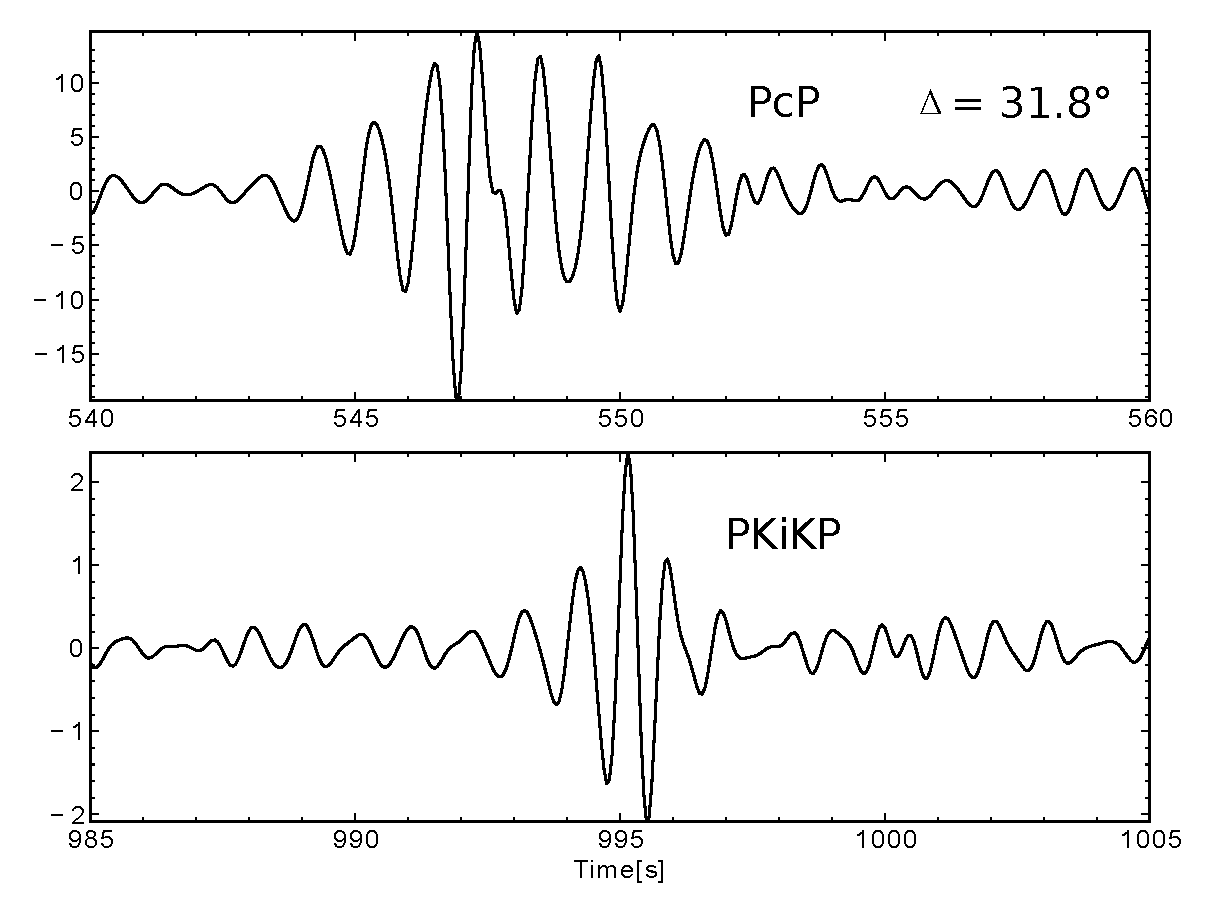
\includegraphics[width=8cm,height=8cm]{fig/chap4/amp_pd_4371355.eps}
}
	\hfill{}
	\caption{NVAR和PDAR记录到的表\ref{nvpd}中事件10产生的PKiKP和PcP信号对比。波形均为%
每个台阵所有台站记录到的对应相位的最大振幅叠加后的结果。(a)为NVAR台阵的记录,上为PcP,下为%
PKiKP;(b)PDAR台阵的记录,上为PcP,下为PKiKP。}
	\label{amp_comp_nvpd_4371355}
\end{figure}
	
表\ref{nvpd}中的事件10产生的PcP在NVAR和PDAR台阵的记录中存在很大差别,而对于PKiKP相位两台阵
之间的差别则很小(图\ref{amp_comp_nvpd_4371355}),使得两个台阵观测到的PKiKP/PcP振幅比分别
为0.03和0.15;图\ref{amp_comp_nvpd_2872958}中则显示,对于事件6,两台阵记录到相似的PcP和PK
iKP波形,振幅比也很接近,分别为0.145和0.143。

\begin{figure}[!ht]
	\hfill{}
	\subfloat[]{\centering%
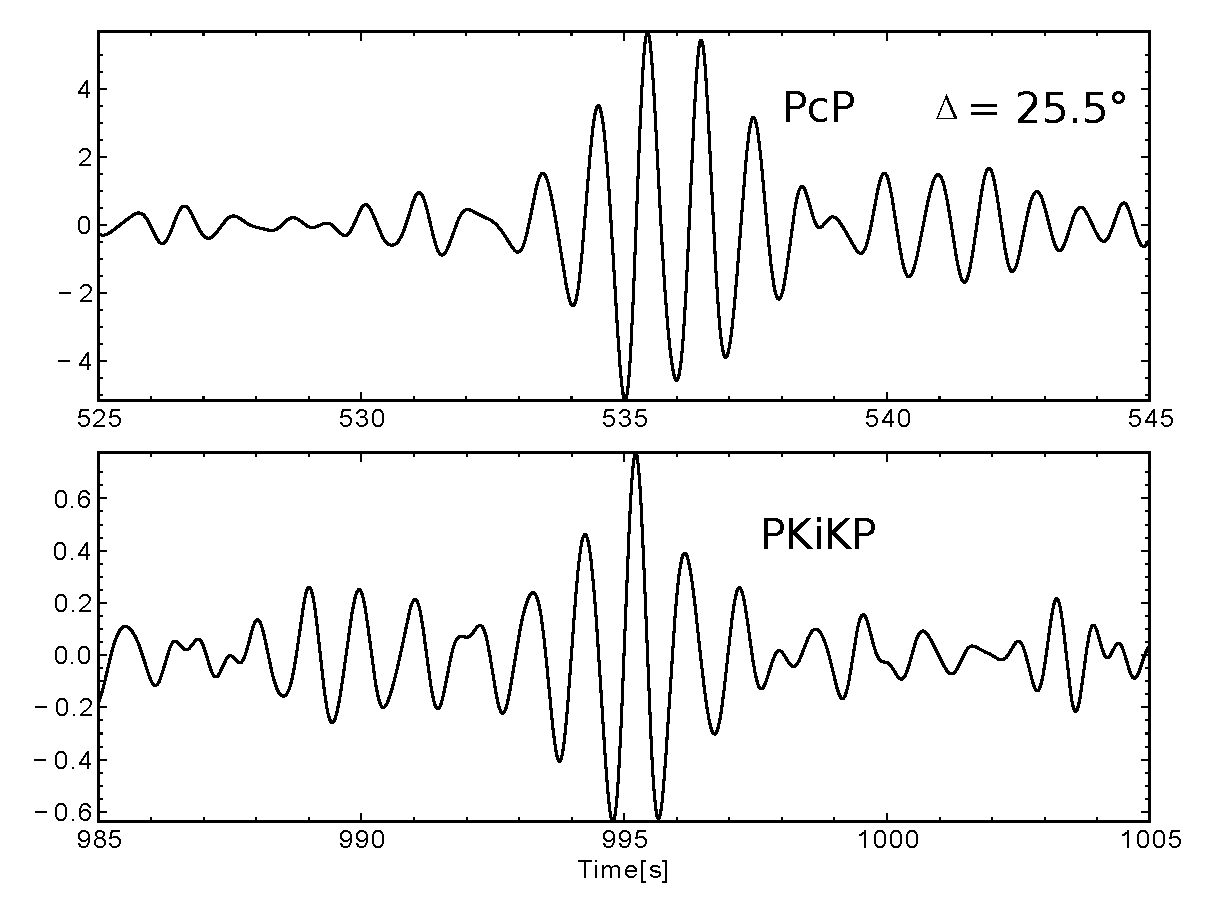
\includegraphics[width=8cm,height=8cm]{fig/chap4/amp_nv_2872958.eps}
}
	\hfill{}
	\subfloat[]{\centering%
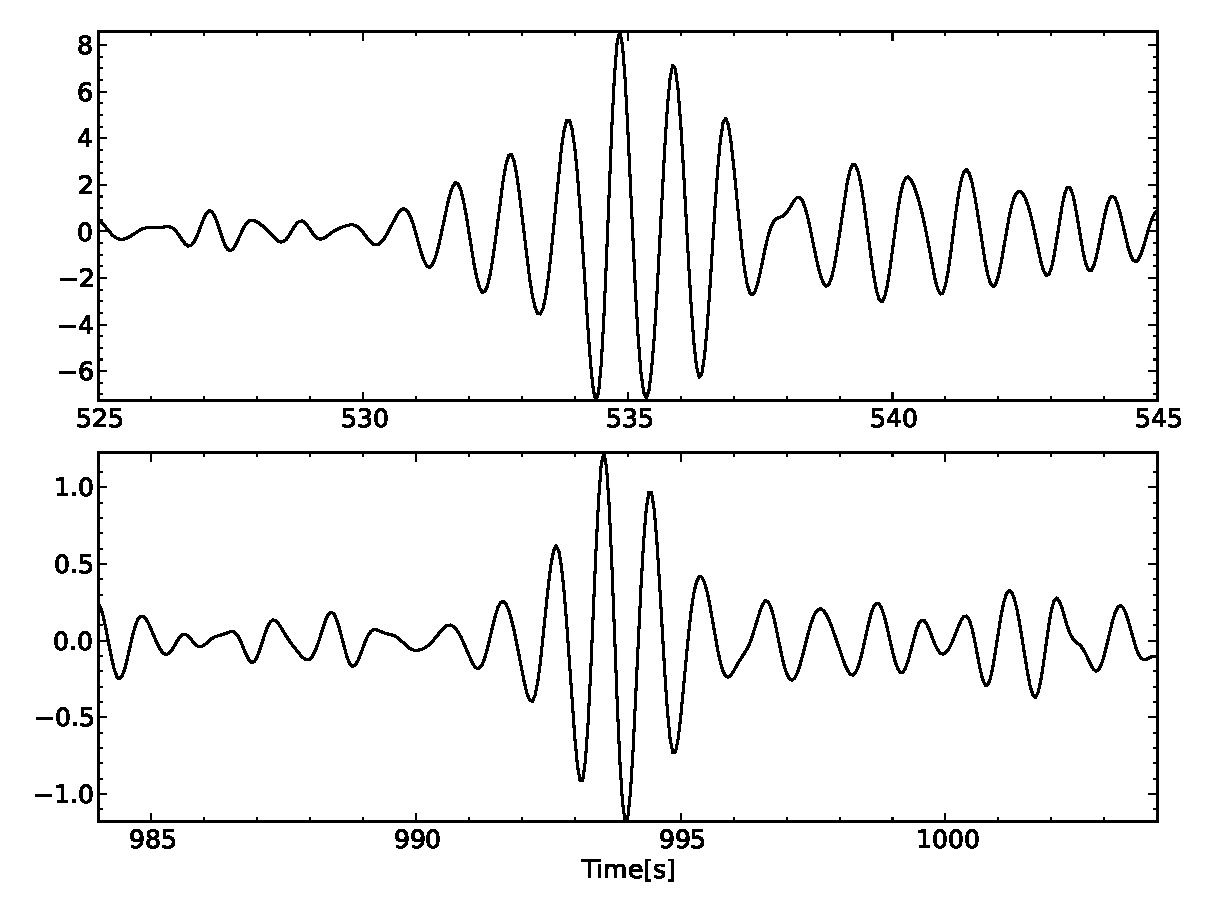
\includegraphics[width=8cm,height=8cm]{fig/chap4/amp_pd_2872958.eps}
}
	\hfill{}
	\caption{NVAR和PDAR记录到的表\ref{nvpd}中事件6产生的PKiKP和PcP信号对比。波形均为%
每个台阵所有台站记录到的对应相位的最大振幅叠加后的结果。(a)为NVAR台阵的记录,上为PcP,下为%
PKiKP;(b)PDAR台阵的记录,上为PcP,下为PKiKP。}
	\label{amp_comp_nvpd_2872958}
\end{figure}

\begin{figure}[!ht]
	\centering
	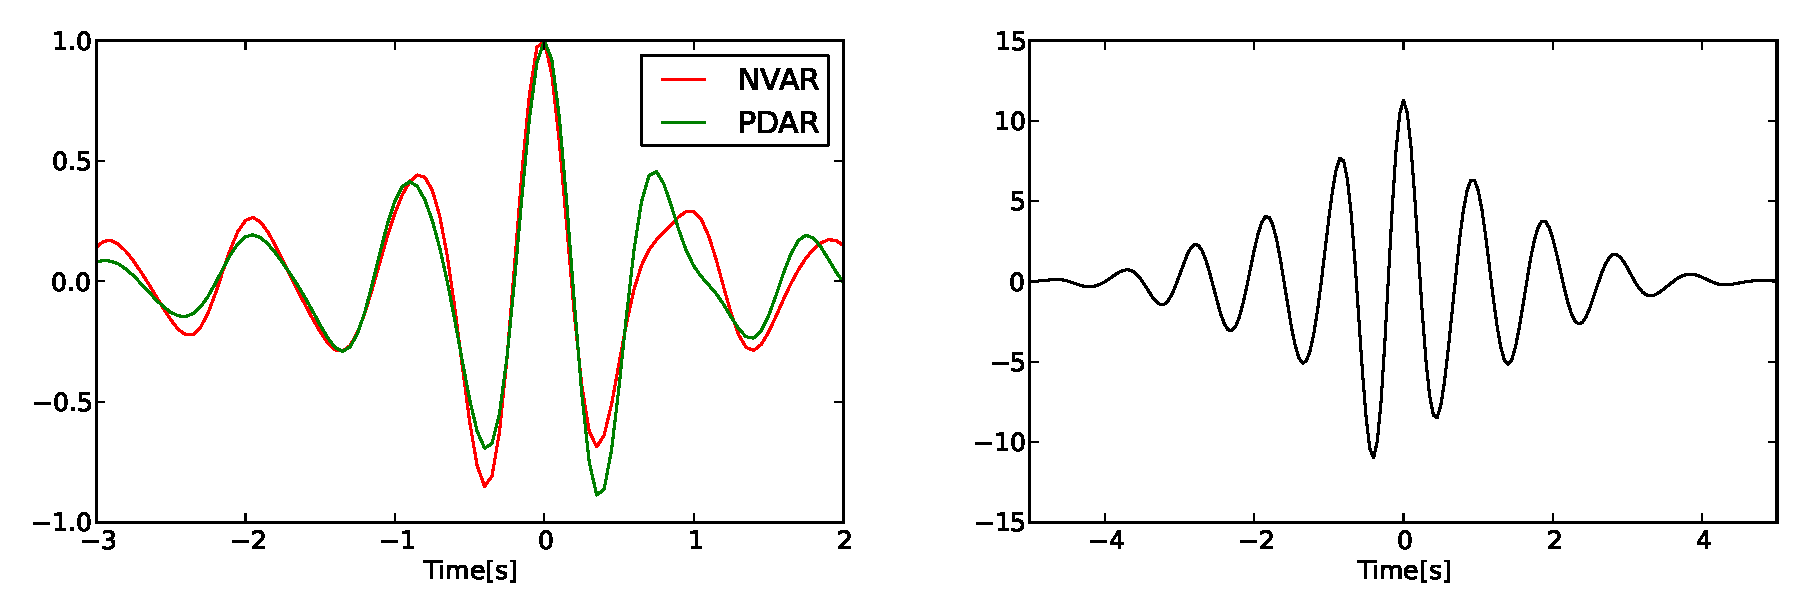
\includegraphics[width=16cm,height=5cm]{fig/chap4/wf_cor.eps}
	\caption{图\ref{amp_comp_nvpd_4371355}中的PKiKP波形比较,左边是将两个波形归一化后%
画在一起,按照各自的最大振幅对齐;右边是归一化后的PKiKP波形的互相关函数。可以看出两个台阵记录到的PKiKP波形相似度非常高,最大互相关值在两个波形的最大振幅处取得。}
	\label{wf_cor}
\end{figure}

从图\ref{amp_comp_nvpd_4371355}中可以发现,NVAR和PDAR记录到的PKiKP信号均很清晰,不仅
振幅很接近,而且波形也很相似,由于是同一地震产生的同一震相,这也是完全符合预期的。但两台阵记录到
的PcP信号却大不相同,NVAR记录中的PcP清晰尖锐,和PKiKP具有相似性,图\ref{wf_cor}是两个PKiKP
波形的互相关;PDAR记录中的PcP前半部分和NVAR记录到的PcP略有相似性,但后半部分还有别的信号成分
,并且PcP振幅只有前者的五分之一左右。异常小的PcP振幅和复杂的PcP波形揭示了PcP在CMB反射点区域存在
复杂的结构特征和强烈的横向变化。很早就有研究发现了来自核慢边界的PKP前驱波,这些前驱波被认为是来自
核慢边界散射~\citep{Bataille1988},散射体的的来源可能有(1)热边界层;(2)化学边界层,即比地幔密
度大但比外核密度小的物质沉积在CMB上或在CMB附近地幔物质和外核物质发生了化学反应形成残留在CMB的
不均匀体;(3)CMB地形的不规则,正如之前提到的,CMB地形的起伏也会减弱反射的PcP振幅。后续又有很多研
究发现了支持CMB存在强烈散射的证据,比如PKKP前驱波的研究~\citep{Rost2010616}等。
图\ref{amp_comp_nvpd_4371355}中PDAR台阵记录到的复杂PcP波形可能是在CMB散射的结果。

再通过对比图\ref{amp_comp_nvpd_4371355}和图\ref{amp_comp_nvpd_2872958},它们对应的两个
事件的震级相同均为5.5,震源深度也仅差10km,可以发现:(1)对于两个事件,NVAR记录到的PcP振幅则相差1
0倍,PKiKP振幅只有两倍的差别;(2)事件6的两个台阵记录的PcP振幅与PDAR记录到的事件10的PcP振幅相
近。(3)对于两个事件,PcP在CMB的反射点距离在200-250km之间,PKiKP在ICB的反射点只有80-90km。
综合这三点可以推测,对于事件6,PcP在核幔边界的反射点可能位于低速带内,虽然台阵到两个事件的震
中距有所差别,且射线路径也不一样,但这些差别不足以解释观测到的巨大的PcP振幅差异和PKiKP振幅大小的
相似性。

\begin{figure}
	\centering
	\includegraphics[width=12cm,height=10cm]{fig/chap4/cmb_bp_loc.eps}
	\caption{NVAR、PDAR台阵和表\ref{nvpd}中所有事件的PcP的CMB反射点位置。事件仅画出%
6和10,对于其余事件仅画出反射点。红色对应较大的PKiKP/PcP振幅,蓝色对应较小的PKiKP/PcP振幅。%
事件10的PcP在CMB反射点的距离约245km,PKiKP在ICB的反射点距离约85km。}
\end{figure}